\documentclass[
	ngerman,
	ruledheaders=section,   % Ebene bis zu der die Überschriften mit Linien abgetrennt werden, vgl. DEMO-TUDaPub
	class=report,		    % Basisdokumentenklasse. Wählt die Korrespondierende KOMA-Script Klasse
	thesis={type=bachelor}, % Dokumententyp Thesis, für Dissertationen siehe die Demo-Datei DEMO-TUDaPhd
	accentcolor=9c,			% Auswahl der Akzentfarbe
	custommargins=false,    % Ränder werden mithilfe von typearea automatisch berechnet
	marginpar=false,        % Kopfzeile und Fußzeile erstrecken sich nicht über die Randnotizspalte
	% BCOR=5mm,             % Bindekorrektur, falls notwendig
	parskip=half-,          % Absatzkennzeichnung durch Abstand vgl. KOMA-Script
	fontsize=11pt,          % Basisschriftgröße laut Corporate Design ist mit 9pt häufig zu klein
]{tudapub}

% Scala support
\usepackage{listings}
\usepackage{color}

\definecolor{dkgreen}{rgb}{0,0.6,0}
\definecolor{gray}{rgb}{0.5,0.5,0.5}
\definecolor{mauve}{rgb}{0.58,0,0.82}

\lstset{
  language=scala,
  aboveskip=3mm,
  belowskip=3mm,
  showstringspaces=false,
  basicstyle={\small\ttfamily},
  numbers=none,
  numberstyle=\tiny\color{gray},
  keywordstyle=\color{blue},
  commentstyle=\color{dkgreen},
  stringstyle=\color{mauve},
  breaklines=true,
  breakatwhitespace=true,
  tabsize=2,
}
 
% Sprachanpassung & Verbesserte Trennregeln 
\usepackage[english, main=ngerman]{babel}

% Anführungszeichen vereinfacht
\usepackage[autostyle]{csquotes}

% Falls mit pdflatex kompiliert wird, wird microtype automatisch geladen, in diesem Fall muss diese Zeile entfernt werden, und falls weiter Optionen hinzugefügt werden sollen, muss dies über
% \PassOptionsToPackage{Optionen}{microtype} vor \documentclass hinzugefügt werden.
\usepackage{microtype}

% Literaturverzeichnis
\usepackage{biblatex} 
\bibliography{DEMO-TUDaBibliography}
 
% Paketvorschläge Tabellen 
\usepackage{tabularx}    % Tabellen, die sich automatisch der Breite anpassen
\usepackage{booktabs}    % Verbesserte Möglichkeiten für Tabellenlayout über horizontale Linien

% Paketvorschläge Mathematik
% \usepackage{mathtools} % erweiterte Fassung von amsmath
% \usepackage{amssymb}   % erweiterter Zeichensatz
% \usepackage{siunitx}   % Einheiten

% Formatierungen für Beispiele in diesem Dokument. Im Allgemeinen nicht notwendig!
\let\file\texttt
\let\code\texttt
\let\tbs\textbackslash
\let\pck\textsf
\let\cls\textsf

% Zapf-Dingbats Symbole
\usepackage{pifont}
\newcommand*{\FeatureTrue }{\ding{52}}
\newcommand*{\FeatureFalse}{\ding{56}}

\begin{document}

\Metadata{
	title=TUDaThesis - Abschlussarbeiten im CD der TU Darmstadt,
	author=Marei Peischl
}

\title{My Bachelorthesis title}
% \subtitle{No subtitle}
\author[P. Hinz]{Philipp Hinz} % optionales Argument ist die Signatur,
\reviewer{Gutachter 1 \and Gutachter 2 \and noch einer \and falls das immernoch nicht reicht}

% Diese Felder werden untereinander auf der Titelseite platziert.
% \department ist eine notwendige Angabe, siehe auch dem Abschnitt `Abweichung von den Vorgaben für die Titelseite'

% Das Kürzel wird automatisch ersetzt und als Studienfach gewählt, siehe Liste der Kürzel im Dokument.
\department{inf}
\institute{Institut}
\group{Arbeitsgruppe}

\submissiondate{\today}
\examdate{\today}

\maketitle

% oder \affidavit[digital] falls eine rein digitale Abgabe vorgesehen ist.
\affidavit
% Es gibt mit Version 3.20 die Möglichkeit ein Bild als Signatur einzubinden.
% TUDa-CI kann nicht garantieren, dass dies zulässig ist oder eine eigenhändige Unterschrift ersetzt.
% Dies ist durch Studierende vor der Verwendung abzuklären.
% Die Verwendung funktioniert so:
%\affidavit[signature-image={\includegraphics[width=\width,height=1cm]{example-image}}, <hier können andere Optionen wie z.B. affidavit=digital zusätzlich stehen>]

\tableofcontents

\chapter{Introduction}
\section{Case Study}

\chapter{Background and Related Work}
\section{Local-First}
\section{CvRDT and CmRDT}
\section{Technical Stack}

\chapter{Extendable Commutative Replicable Data Types}
In this chapter we will introduce the concept of Extendable Commutative Replicable Data Types (ECmRDT) and present our implementation of this concept.

\section{Motivation}
CvRDTs and CmRDTs do not care about authentication and authorization. This is usally not a problem in trusted environments like a cluster of servers. But used in client running applications (local-first applications) we usally can not trust our clients. Therefore we need to add authentication and authorization to our data types. 

Additionally local-first applications require end-to-end encryption if we want to store our data on a server. This is usally difficult to combine with authentication and authorization. 

Our here proposed solution is specially designed for a single server, but the concepts can be easily applied to peer-to-peer applications. We explore the use in peer-to-peer applications a bit in the future work section.

Initially we tried to design a CRDT specifically for authentication and authorization. But we found out that a more abstract approach is more flexible and easier to implement. Therefore we designed a new data type called Extendable Commutative Replicable Data Type (ECmRDT) with authentication and authorization as an extension.

\section{Overview}
We base our \code{ECmRDT} on CmRDTs and therefore make use of event sourcing. Because we design our \code{ECmRDT} to be used in server/client applications we only use direct event sourcing in storing the \code{Event}s on the server. On the client we use a more classic approach and only store the last state of the data type and all pending events to be sent to the server. Incoming events are applied to the last state to get the new state.

The core feature of our \code{ECmRDT} is the concept of extensions. Extensions are a way to add functionality by mutation of state through events or validation of events. 

\subsection{Concepts}

In this chapter, we will introduce the concepts of our \code{ECmRDT} with definitions and code examples.

\minisec{ReplicaId}
The \code{ReplicaId} is a unique identifier for a replica / the user. The \code{ReplicaId} is in our case a public key. We will go into detail why we use a public key as \code{ReplicaId} in our chapter about authentication and authentication.

\begin{lstlisting}
case class ReplicaId(
  val publicKey: BinaryData
)
\end{lstlisting}

\minisec{AggregateId}
The \code{AggregateId} is a unique identifier for an \code{ECmRDT}. The \code{AggregateId} is a combination of a \code{ReplicaId} and some random bytes. The \code{ReplicaId} is the \code{ownerReplicaId} of the Aggregate. The random bytes are used to prevent collisions of \code{AggregateId}s.

\begin{lstlisting}
case class AggregateId(
  val replicaId: ReplicaId,
  val randomBytes: BinaryData
)
\end{lstlisting}

\minisec{Effect}
An \code{Effect} is a function that takes a \code{state}, an context, an \code{MetaContext} and returns a new \code{state} or an \code{RatableError} in future. By returning an \code{RatableError} we can verify the \code{Event} together with the given parameters. The effect is an asynchronous operation because we need to use cryptograpic operations to verify the \code{Event} which are usally implemented asynchronously.

\begin{lstlisting}
type Effect[A, C] = (A, C, MetaContext) => EitherT[Future, RatableError, A]
\end{lstlisting}

\minisec{Event}
If the user wants to take any actions on the \code{ECmRDT}, he has to create an event. Every event is associated with a context. An \code{Event} is applied to the \code{ECmRDT} by converting it into an \code{Effect}.

\begin{lstlisting}
trait Event[A, C]:
  def asEffect: Effect[A, C]
\end{lstlisting}

\minisec{MetaContext}
The \code{MetaContext} is a context that is passed to the \code{ECmRDT} when applying an \code{Event}. It contains information about the \code{ownerReplicaId} and the \code{aggregateId}. 

The need results from the fact, that the initialization of \code{ECmRDT}s also happens through an \code{Event}. While processing the first \code{Event} we do not have any \code{state} yet. Therefore we could normally not validate the \code{Event}. The \code{MetaContext} is mainly used to validate the first \code{Event} by checking if the \code{Event} was created by the \code{ownerReplicaId}.

\begin{lstlisting}
case class MetaContext(
  val aggregateId: AggregateId,
  val ownerReplicaId: ReplicaId,
)
\end{lstlisting}

\minisec{ECmRDTEventWrapper}
The \code{ECmRDTEventWrapper} is a wrapper for an \code{Event} and a context. It is used to bundle the \code{Event} with the context and the \code{clock} of the \code{ECmRDT} when the \code{Event} was created. The \code{clock} is used to prevent duplications of \code{Event}s.

\begin{lstlisting}
case class ECmRDTEventWrapper[A, C, +E <: Event[A, C]](
  val time: Long,
  val event: E,
  val context: C,
)
\end{lstlisting}

\minisec{Context}
The context contains meta information about a single \code{Event} but is the same for all \code{Event}s of a single \code{ECmRDT} implementation. The idea is to compose the context out of multiple traits.

An core context trait is the \code{IdentityContext}. This context trait is always required and contains the \code{ReplicaId} of the creator of this \code{Event}. The validation of this identity is not done by the \code{ECmRDT} but must be done externally. More on this in the section about authentication and authorization.

\begin{lstlisting}
trait IdentityContext:
	def replicaId: ReplicaId
\end{lstlisting}

\minisec{ECmRDT}
Our core concept is the \code{ECmRDT}. The \code{ECmRDT} consists of a \code{state} and a \code{clock}. The \code{state} is the actual data of the \code{ECmRDT}. The \code{clock} is a \code{VectorClock} to prevent duplications of \code{Event}s. Our \code{ECmRDT} does not handle distribution of \code{Event}s nor storing pending \code{Event}s. This has to be done by the user of the \code{ECmRDT}.

Our \code{ECmRDT} supports two operations. One to \code{prepare} an \code{Event} and one to apply an prepared event called \code{ECmRDTEventWrapper}. The \code{prepare} operation is used to aquire additional information from the \code{ECmRDT}, specifically the \code{clock} and bundle the event with an context into one \code{ECmRDTEventWrapper}. The \code{apply} operation is used to apply the \code{Event} to the \code{ECmRDT}.

\begin{lstlisting}
case class ECmRDT[A, C <: IdentityContext, E <: Event[A, C]](
	val state: A,
	val clock: VectorClock = VectorClock(Map.empty)
):
	def prepare(
		event: E, context: C
	)(
		using effectPipeline: EffectPipeline[A, C]
	): ECmRDTEventWrapper[A, C, E] = ...

	def effect(
		wrapper: ECmRDTEventWrapper[A, C, E], meta: MetaContext
	)(
		using effectPipeline: EffectPipeline[A, C]
	): EitherT[Future, RatableError, ECmRDT[A, C, E]] = ...
\end{lstlisting}

\minisec{EffectPipeline}
The \code{EffectPipeline} is a simple structure that converts an existing \code{Effect} into a new \code{Effect}. It is the core piece in implementing extensions. The \code{EffectPipeline} is implicitly specified by a \code{ECmRDT} implementation and is used to implement additional functionality like logging, validation or mutation. Functionality provided by the \code{EffectPipeline} is applied to all \code{Event}s of a \code{ECmRDT}.

\begin{lstlisting}
trait EffectPipeline[A, C]:
	def apply(effect: Effect[A, C]): Effect[A, C]
\end{lstlisting}

\subsection{Usage and Example}
The usage of an \code{ECmRDT} is generally simple. The user has to specify an State, a Context, some \code{Event}s and a \code{EffectPipeline}. 

When the user wants to apply an \code{Event} with an Context, he first has to prepare it. The preparation will add an time to the \code{Event} and bundle it with the Context. The user can then apply the prepared \code{Event} to the \code{ECmRDT}. 

To apply the prepared event it is first converted into an \code{Effect}. This \code{Effect} is then converted into a new \code{Effect} by the \code{EffectPipeline}. With all provided information the \code{ECmRDT} can then convert its previous \code{state} using the \code{Effect} into a new \code{state}. The \code{state} with an updated \code{VectorClock} is then returned to the user.

An minimal example of an \code{ECmRDT} implementation is shown in the following listing. The \code{ECmRDT} is a simple counter that can be incremented.

\begin{lstlisting}
case class CounterState(value: Int)

// Empty pipeline because we don't need any extensions
object CounterState:
  given EffectPipeline[Counter, CounterContext] = EffectPipeline()

case class CounterContext(replicaId: ReplicaId) extends IdentityContext

sealed trait CounterEvent extends Event[CounterState, CounterContext]

case class IncrementEvent() extends CounterEvent:
	def asEffect: Effect[CounterState, CounterContext] =
		(state, context, meta) => state.copy(value = state.value + 1)

// Somewhere in user code
val counter = ECmRDT[CounterState, CounterContext, CounterEvent](CounterState())

\end{lstlisting}

\subsection{Extensions}

The most important new feature of ECmRDTs and the reason for Contexts to exist is the ability to extend the functionality of an ECmRDT. The idea is, that an extension can define a new Context trait or new State trait and then implement the \code{EffectPipeline}. While defining the \code{EffectPipeline} the extension can specify its required traits or traits from other extensions as type bounds. This allows to build extensions onto each other. The EffectPipeline can then use the traits to implement either validation or also mutation of the state.

An minimal extension that counts the number of events could looks like this.

\begin{lstlisting}

trait CountEventsState:
	// We define attributes as methods. This later allows
	// us to override them as attributes
	def count: Int

object CountEventsEffectPipeline:
	def apply[A <: CountEventsState, C](): EffectPipeline[A, C] =
		(effect) => (state, context, meta) =>
			for 
				newState <- effect(state, context, meta)
			yield
				newState.copy(count = newState.count + 1)

\end{lstlisting}

We could define an additional extension that logs all events.

\begin{lstlisting}

object LoggingEffectPipeline:
	def apply[A <: CountEventsState, C](): EffectPipeline[A, C] =
		(effect) => (state, context, meta) =>
			for
				newState <- effect(state, context, meta)
			yield
				println(s"Event ${meta.event} applied by ${context.replicaId}")
				newState

\end{lstlisting}

In our earlier example we could now use both extensions like this.

\begin{lstlisting}

case class CounterState(
	value: Int,
	count: Int // We can now easily override as attribute
) extends CountEventsState:

object CounterState:
  given EffectPipeline[Counter, CounterContext] = EffectPipeline(
		// We can now use both extensions
		// They will later be used implicitly by the ECmRDT
		CountEventsEffectPipeline(),
		LoggingEffectPipeline()
  )

\end{lstlisting}

\section{Authentication and Authorization}

Now that we have proposed the design of our ECmRDT we can come back to the problem of authentication and authorization. Our primary goal is to be able to check for an event sent by an user if the user is allowed use the event. 

We solved this issue by defining new concepts called \code{Claim}, \code{ClaimProof} and \code{ClaimProver} using asymmetric cryptography. For every \code{Claim} there always exist exactly one \code{ClaimProver} and multiple \code{ClaimProof}s. The \code{Claim} is a public key that is used to verify the signature in the \code{ClaimProof}. An \code{ClaimProof} is a signature of the \code{ReplicaId} by the sender signed with a private key contained in the \code{ClaimProver}. Because \code{ClaimProof} only contains an signature, the \code{Claim} and \code{ClaimProof} are considered to be public information. 

The concepts are used in the following way. All \code{Claim}s are publicly saved in the \code{state} of the \code{ECmRDT}. Every event contains a set of \code{ClaimProof}s. Now every event will define in advance which \code{Claim}s are required to be present in the \code{ClaimProof}s. An EffectPipeline can then check if all provided \code{ClaimProof}s are valid. 

\minisec{Claim vs ReplicaId}

This approach lets one thing open. How can we ensure that the \code{ReplicaId} in the \code{ClaimProof} is the same as the \code{ReplicaId} of the sender?

This issue is solved by the definition of the \code{ReplicaId} itself. An \code{ReplicaId} is an asymmetric public key. When a user wants to send an event he first creates a signature of the event with his private key. This signature is then sent with the event. The \code{ReplicaId} is then used to verify the signature. Therefore everyone can verify that the event was sent by the user with the \code{ReplicaId} and that the \code{ReplicaId} is the same as the one in the \code{ClaimProof}.

One might ask why we don't just save a set of \code{ReplicaId}s in the \code{state} instead of \code{Claim}s. This is actually the recommended way if the use case allows it. The reason why we use \code{Claim}s is that we want users to be able to aquire authorization at any time using a piece of information. We actually later show a way to reduce the amount of information needed to a short password. The approach of using \code{ReplicaId}s is more suitable for use cases where the authorization is granted by users.

\minisec{Read Access}

The here proposed approach is very flexible. While it would be possible to restrict read access we did not need it in our use case. Therefore we did not implement it but will show how it could be done in the future work section.

\newpage

\subsection{Example}

We want to extend our previously defined \code{Counter} with the ability to restrict access to the \code{IncrementEvent}. For this we have define an \code{CounterClaimEnum} to idenify \code{Claim}s, extend the \code{CounterState} to contain a set of \code{Claim}s and extend the \code{CounterContext} to contain a set of \code{ClaimProof}s. Additionally we have to install a new \code{EffectPipeline} that checks if the \code{ClaimProof}s are valid and check for the needed claims in the event.

\begin{lstlisting}

enum CounterClaimEnum:
	case Increment

case class CounterState(
	value: Int,
	count: Int,
	claims: Set[Claim[CounterClaimEnum]]
) extends CountEventsState

case class CounterContext(
	replicaId: ReplicaId,
	claimProofs: Set[ClaimProof[CounterClaimEnum]]
) extends CountEventsContext

object CounterState:
	given EffectPipeline[Counter, CounterContext] = EffectPipeline(
		CountEventsEffectPipeline(),
		LoggingEffectPipeline(),
		// We install a new EffectPipeline that checks if the ClaimProofs are valid
		AsymPermissionEffectPipeline[CounterState, CounterClaimEnum, CounterContext]
	)

sealed trait CounterEvent extends Event[CounterState, CounterContext]

case class IncrementEvent() extends CounterEvent:
	def asEffect: Effect[CounterState, CounterContext] =
		(state, context, meta) =>
			for
				newState <- context.verifyClaim(CounterClaimEnum.Increment)
			yield
				newState.copy(count = newState.count + 1)

\end{lstlisting}

\newpage

This definition could now be used in the following way.

\begin{lstlisting}

def main(using Crypt) = 
  for
    replicaId <- EitherT.liftF(PrivateReplicaId())

    // Step 1: Create claims and claimProvers.
    claimsPair <- EitherT.liftF(
      Claim.create(List(CounterClaimEnum.Increment))
    )

    (claims, provers) = claimsPair

    proof <- EitherT.liftF(
      provers.head.prove(replicaId)
    )

    // Step 2: Create initial state.
    counter = ECmRDT[CounterState, CounterContext, CounterEvent](CounterState(0, claims))

    // Step 3: Create event.
    eventPrepared = counter.prepare(
      IncrementEvent(),
      CounterContext(replicaId, List(proof))
    )

    // Step 4: Verify and advance state.
    newCounter <- counter.effect(eventPrepared, MetaContext(null, null))

  yield
    println(s"New counter: \${newCounter.state.value}") // 1

\end{lstlisting}

\section{ECmRDT Example}
\section{Conclusion}

\chapter{Ratable}
In this chapter we will look into how Ratable is implemented and how concepts from the previous chapter are used.

\section{Architecture}
Ratable consists of three main parts. The Core, the Functions and the Webapp. The Webapp is the interface to the user. Using ECmRDTs, our Webapp contains most of our application logic and our state. The Functions are the backend of our Webapp. They are responsible for storing and passing Events to and from the Webapp. The Core is shared between the Webapp and the Functions. It contains the ECmRDT library and all of the ECmRDT aggregates.

The communication between our Webapp and our Functions works in two ways. Since we want to pass Events to the Functions in realtime, we have to use a websocket connection. Additionally for synchronous requests we use a REST API. The communication protocol uses Protobufs. We are not using JSON because we use a lot of 'oneof' relationships in our data and Scala 3 json libraries do not satisfactorily support this.

The two main projects Functions and Webapp are structured similarly. The most central aspect to our design is seperation into multiple layers of modules and heavy usage of dependency injection to allow for easy testing and modularization.

Both projects consist of a root layer, an application layer, a device layer and multiple other layers. This structure can be thought of similarly to a tree as shown in figure \ref{fig:architecture}. Every layer contains services and other modules. The device layer abstracts over the underlying platform. This allows us to mock it and test the rest of the application. The root layer contains core services and modules like logging or configuration. The application layer is the core of both projects containing important logic specific two each project.

\begin{figure}[htbp]
\centering
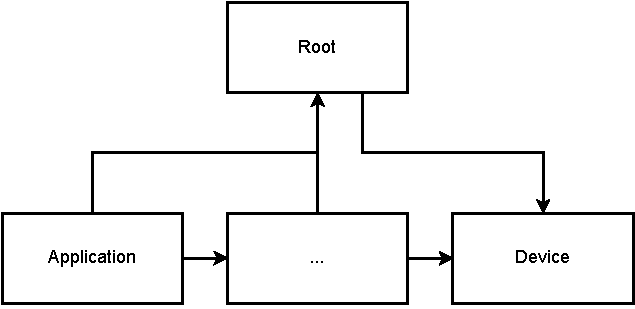
\includegraphics[width=0.8\textwidth]{architecture_1.pdf}
\caption{Architecture}
\label{fig:architecture}
\end{figure}

\minisec{Dependency Injection}

We implemented dependency injection by structural typing. This allows us to inject services in the following way.

\begin{lstlisting}
class MyService(services: {
	val myDependency: MyDependency
}):
	def doSomething() = ???

class MyDependency(services: {})

class Services:
	lazy val myService = new MyService(this)
	lazy val myDependency = new MyDependency(this)

// ...

val services = new Services()
services.myService.doSomething()

\end{lstlisting}

\section{Core}
The Core contains three big parts. The ECmRDT library and some additionally needed definitions, the ECmRDT aggregates containing the actual domain logic and the protobuf definitions defining the communication protocol between the Webapp and the Functions.

The actual domain is for our use case very small and will show how the ECmRDT library can be used to implement a simple application.

\minisec{Domain - Ratable}

The state is pretty simple. We have a Ratable containing a title, a list of categories and a list of ratings. Additionally for our extensions we define claims and claimsBehindPassword. Note here, that the State can and should already contain domain logic. 

\begin{lstlisting}

case class Category(
  val title: String
)

case class Rating(
  val ratingForCategory: Map[Int, Int]
)

enum RatableClaims extends Enum[RatableClaims]:
  case CanRate

case class Ratable(
  val claims: List[Claim[RatableClaims]],
  val claimsBehindPassword: Map[RatableClaims, BinaryDataWithIV],

  val title: String,
  val categories: Map[Int, Category],
  val ratings: Map[ReplicaId, Rating]
)
extends AsymPermissionStateExtension[RatableClaims], ClaimByPasswordStateExtension[RatableClaims]:
	def rate(replicaId: ReplicaId, ratingForCategory: Map[Int, Int]): Ratable = ???

	def categoriesWithRating: Map[Int, (Category, Int)] = ???

\end{lstlisting}

\begin{lstlisting}

object Ratable:
  given (using Crypt): EffectPipeline[Ratable, RatableContext] = EffectPipeline(
    AsymPermissionEffectPipeline[Ratable, RatableClaims, RatableContext]
  )

  given InitialECmRDT[Ratable] = InitialECmRDT(Ratable(
    List(), Map(), "missing-title", Map(0 -> Category("missing-categories")), Map()
  ))

\end{lstlisting}

\begin{lstlisting}

case class RatableContext(
	val replicaId: ReplicaId,
	val proofs: List[ClaimProof[RatableClaims]]
	) 
	extends IdentityContext 
		with AsymPermissionContextExtension[RatableClaims]

\end{lstlisting}

\begin{lstlisting}

sealed trait RatableEvent extends Event[Ratable, RatableContext]

case class RateEvent(
  val ratingForCategory: Map[Int, Int]
) extends RatableEvent:
  def asEffect: Effect[Ratable, RatableContext] =
    (state, context, meta) =>
      for
        _ <- context.verifyClaim(RatableClaims.CanRate)
        _ <- EitherT.cond(ratingForCategory.size == state.categories.size, (),
          RatableError(s"Rating must contain ${state.categories.size} categories, but ${ratingForCategory.size} given"))
      yield
        state.rate(context.replicaId, ratingForCategory)


case class CreateRatableEvent(
  val canRate: Claim[RatableClaims],
  val canRateBehindPassword: BinaryDataWithIV,

  val title: String,
  val categories: List[String]  
) extends RatableEvent:
  def asEffect: Effect[Ratable, RatableContext] =
    (state, context, meta) =>
      for
        _ <- EitherT.cond(meta.ownerReplicaId == context.replicaId, (),
          RatableError(s"Replica ${context.replicaId} is not the owner ${meta.ownerReplicaId} of this object."))
        
      yield
        Ratable(
          List(canRate),
          Map(RatableClaims.CanRate -> canRateBehindPassword),
          title,
          categories
            .zipWithIndex
            .map((title, index) => (index, Category(title)))
            .toMap,
          Map()
        )
		
\end{lstlisting}

\begin{lstlisting}

case class CreateRatableResult(
  val event: CreateRatableEvent,
  val password: String
)

def createRatable(title: String, categories: List[String])(using crypt: Crypt): Future[CreateRatableResult] =
  val password = Random.alphanumeric.take(18).mkString

  for
    (canRateClaim, canRateProver) <- Claim.create(RatableClaims.CanRate)
    claimBehindPassword <- ClaimBehindPassword(canRateProver.privateKey.inner, password)

  yield
    CreateRatableResult(
      CreateRatableEvent(
        canRateClaim,
        claimBehindPassword,
        title,
        categories
      ),
      password
    )

\end{lstlisting}

\minisec{Protobuf}


\section{Functions}
Our goal was to use similar technologies in front and backend. Additionally, our goal was to use cloud services as much as possible. Therefore, we decided to use the serverless approach provided by Azure Functions. This is especially useful because the cost of small projects is very low. Additionally, we can easily scale up if needed.

Azure functions provide a lot of different languages to implement them including JVM languages and Javascript. We decided to use Javascript because the JVM implementation does not support WebPubSubs yet.

It is possible with scalajs to compile Scala to multiple Javascript files but because of lack of documentation for scala 3 we decided to deploy everything in one single file. Because we still need to provide Azure Functions as multiple Javascript files, we decided to use a proxy approach. Each of the functions is a proxy to the main file. The main file now contains two gateways that handle the messages using a message handler for each message type.

The first gateway is the Http gateway. This gateway is used to handle Http requests. This is especially useful for synchronous requests where the user is waiting for a response like login or requesting data. The second gateway is the socket gateway. This gateway is used to handle messages from our WebPubSub send via WebSockets. Contrary to the Http gateway, this gateway is used for asynchronous messages. This is useful for messages like sending or receiving events in real time.

Because we need to use Javascript libraries to interact with our Azure services we abstract them away in our device layer. This allows us to test each of our message handlers without the need to use the Azure services. 

\minisec{ECmRDT}
Different from our WebApp implementation, the state management in our functions is minimal. Because we only need to distribute the events between our clients, we only need to store the events and not act on them. Especially in an end-to-end encryption scenario, acting on the events would not even be fully possible.

\section{Webapp}
WebApp is the primary part of Ratable. It is our interface to Ratables while also containing and handling all logic. It can be thought of similarly to a Frontend combined with a Backend.

\subsection{Application Layer}
The application layer implements the user interface and interactions with the state. 

We tried to approach the WebApp in a use-case-oriented approach. This allows us to easily write tests for each use case and test all scenarios through the whole application. The application layer is split into pages and use-cases. Use cases are called directly by pages and are the only way to manipulate the state from the application layer. Additionally, we provide localization, routing and popups through services.

\subsection{State Layer}
The state layer provides access to the state, distributes it and stores it in the local database. 

All state is accessible through a root layer service providing a simplified interface. The application state is bundled from multiple so called aggregate view repositories types as shown in the following listing.

\begin{lstlisting}

case class ApplicationState(
  ratables: AggregateViewRepository[
    Ratable, RatableContext, RatableEvent
  ],
  library: AggregateViewRepository[
    RatableLibrary, RatableLibraryContext, RatableLibraryEvent
  ]
)

\end{lstlisting}

The goal of an aggregate view repository is to provide a repository for views of one aggregate type. In our case, a repository allows us to get, add and remove views of one aggregate type. It should be noted, getting a view does not only return the view to its current state but also provides all changes to the view in the future.

\begin{lstlisting}

trait AggregateViewRepository[A : InitialECmRDT, C, E <: Event[A, C]]:
  def all: Future[Seq[(AggregateGid, A)]]
  
  def create(id: AggregateId): AggregateView[A, C, E]
  def get(id: AggregateId): EitherT[Future, RatableError, Option[AggregateView[A, C, E]]]

\end{lstlisting}

An aggregate is represented by views and facades. Views are provided publicly to the outside of the state layer and allow us to listen for changes and trigger events. 

\begin{lstlisting}

trait AggregateView[A, C, E <: Event[A, C]]:
  def effect(event: E, context: C)(using EffectPipeline[A, C]): EitherT[Future, RatableError, Unit]
  def listen: Signal[A]

\end{lstlisting}

Facades are used internally and allow broader access to the aggregate. Facades allow us to manipulate the ECmRDT of our aggregate without restrictions and listen to changes to the ECmRDT instead of the aggregate only. This is especially needed to implement the synchronization of the ECmRDT. It should be noted that the AggregateFacade is the place where the ECmRDT is stored.

\begin{lstlisting}

class AggregateFacade[A, C <: IdentityContext, E <: Event[A, C]](
  private val initial: EventBufferContainer[A, C, E]
):
  private val variable = Var(initial)
  private var aggregateInFuture = Future.successful(initial)

  def listen: Signal[EventBufferContainer[A, C, E]] = variable

  def mutateTrivial(
    f: EventBufferContainer[A, C, E] => EventBufferContainer[A, C, E]
  ): EitherT[Future, RatableError, EventBufferContainer[A, C, E]] =
    mutate(aggregate => EitherT.rightT(f(aggregate)))

  def mutate(
    f: EventBufferContainer[A, C, E] => 
      EitherT[Future, RatableError, EventBufferContainer[A, C, E]]
  ): EitherT[Future, RatableError, EventBufferContainer[A, C, E]] = ???

\end{lstlisting}

One might wonder why the AggregateFacade works with EventBufferContainer and not ECmRDTs directly. This is because ECmRDT does not provide storage for events out of the box. This is needed to be able to distribute the events to the server in case of failure. Therefore, we created a wrapper for our ECmRDT that saves all events that are applied to it while also providing a method to acknowledge and remove all events that are successfully distributed. 

\section{Implementation}
\section{Evaluation}

\chapter{Future Work}
\section{Ratable}
\section{ECmRDT}

\printbibliography

\end{document}
